%<dscrpt>Algorithme de Gregory.</dscrpt>
Dans l'intervalle $I=\left]0,\frac{\pi}{2} \right[$, on définit des fonctions $a$ et $b$ par:
\begin{displaymath}
  \forall \theta\in I,\; a(\theta) = \frac{\theta}{\tan \theta}, \hspace{0.5cm} b(\theta) = \frac{\theta}{\sin \theta}
\end{displaymath}
\begin{figure}[h]
  \centering
  \includegraphics{./Egregory_1.pdf}
  % Egregory_1.pdf: 0x0 pixel, 300dpi, 0.00x0.00 cm, bb=
  \caption{Interprétation géométrique}
  \label{fig: Egregory_1}
\end{figure}

\begin{enumerate}
  \item Encadrement et interprétation géométrique. 
  \begin{enumerate}
    \item Montrer que $0< 2\sin(\frac{\alpha}{2}) < \tan(\alpha)$ pour tous les $\alpha\in I$.
    \item Pour $\alpha \in I$ et $z$ comme sur la figure \ref{fig: Egregory_1}, calculer $|e^{i\alpha} -1|$ et l'affixe $z$. En déduire une interprétation géométrique de l'inégalité de la question a.
  \end{enumerate}

  \item La méthode d'Euclide pour approcher $\frac{\pi}{4}$ consiste à calculer la longueur du polygone régulier inscrit dans l'arc de cercle (le huitième de cercle) en doublant à chaque fois les points.
  
\begin{figure}[h]
  \centering
  \subfloat[initialisation]{\label{fig: Egregory_2}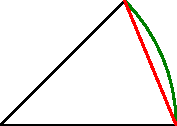
\includegraphics{./Egregory_2.pdf}}
    \hspace{5pt}
  \subfloat[étape 1]{\label{fig: Egregory_3}\includegraphics{./Egregory_3.pdf}}
    \hspace{5pt}
  \subfloat[étape 2]{\label{fig: Egregory_4}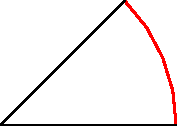
\includegraphics{./Egregory_4.pdf}}
  \caption{Approximation d'Euclide}
\end{figure}
Quelle est l'expression de l'approximation à l'étape $n$? On la notera $e_n$.

  \item Montrer que, pour tous les $\theta\in \left]0,\frac{\pi}{4} \right[$,
\begin{displaymath}
  \frac{1}{\tan \theta} = \frac{1}{\tan 2\theta} + \frac{1}{\sin 2\theta},\hspace{0.5cm}
  \sin \theta = \sqrt{\frac{(\sin 2\theta)\, (\tan \theta)}{2}}
\end{displaymath}

\item Récurrence de Gregory\footnote{James Gregory (1638-1675)}. 
Pour un $\alpha\in I$ fixé et $n\in \N$, on note 
\begin{displaymath}
  a_n = a(\frac{\alpha}{2^{n}}),\hspace{1cm} b_n = b(\frac{\alpha}{2^{n}})
\end{displaymath}
\begin{enumerate}
  \item Montrer que ces suites vérifient les relations de récurrence:
\begin{displaymath}
  a_{n+1} = \frac{1}{2}\left( a_n + b_n\right), \hspace{1cm} b_{n+1} = \sqrt{a_{n+1}b_n} 
\end{displaymath}
  \item En admettant que $1$ est la limite en $0$ des fonctions $a$ et $b$, expliquer comment ces formules de récurrence permettent de mettre en \oe{}uvre une variante de la méthode d'approximation d'Euclide.
\end{enumerate}

\item
\begin{enumerate}
  \item Former des relations analogues à celles de la question 3. pour les fonctions de trigonométrie hyperbolique $\th$ et $\sh$.
  \item Calculer $\th(\ln(2))$ et $\sh(\ln(2))$.
  \item On définit des suites $\left( a_n\right)_{n\in \N}$ et $\left( b_n\right)_{n\in \N}$ par:
\begin{displaymath}
  \left\lbrace 
  \begin{aligned}
    &a_0 = 5 \\ &b_0 = 4
  \end{aligned}
\right. , \hspace{1cm} \forall n\in \N:\;
\left\lbrace 
\begin{aligned}
  a_{n+1} &= \frac{1}{2}\left( a_n + b_n\right)\\ b_{n+1} &= \sqrt{a_{n+1}b_n} 
\end{aligned}
\right. 
\end{displaymath}
Préciser les expressions de $a_n$ et $b_n$ et la limite de ces suites. On admettra que $1$ est la limite en $0$ des analogues hyperboliques de $a$ et $b$. 
\end{enumerate}

\end{enumerate}
